% !TEX root = ../main.tex
\section{Hierarchical Variational Models}
For studying models with correlated random variables, such as frustrated spin systems~\citep{zdeborova2016statistical}, unstructured variational families such as the mean field are insufficient. \Acrfullpl{hvm} are one way to model correlated latent variables. An \gls{hvm} is defined by placing a `variational prior' on the variational parameters $\mbnu$ of the mean field variational family, in analogy to hierarchical probabilistic models. By leveraging neural networks to parameterize the variational prior, \glspl{hvm} can capture complex dependencies between random variables~\citep{ranganath2018black}.

% !TEX root = ../../main.tex
\begin{figure}[t!]
  \centering
  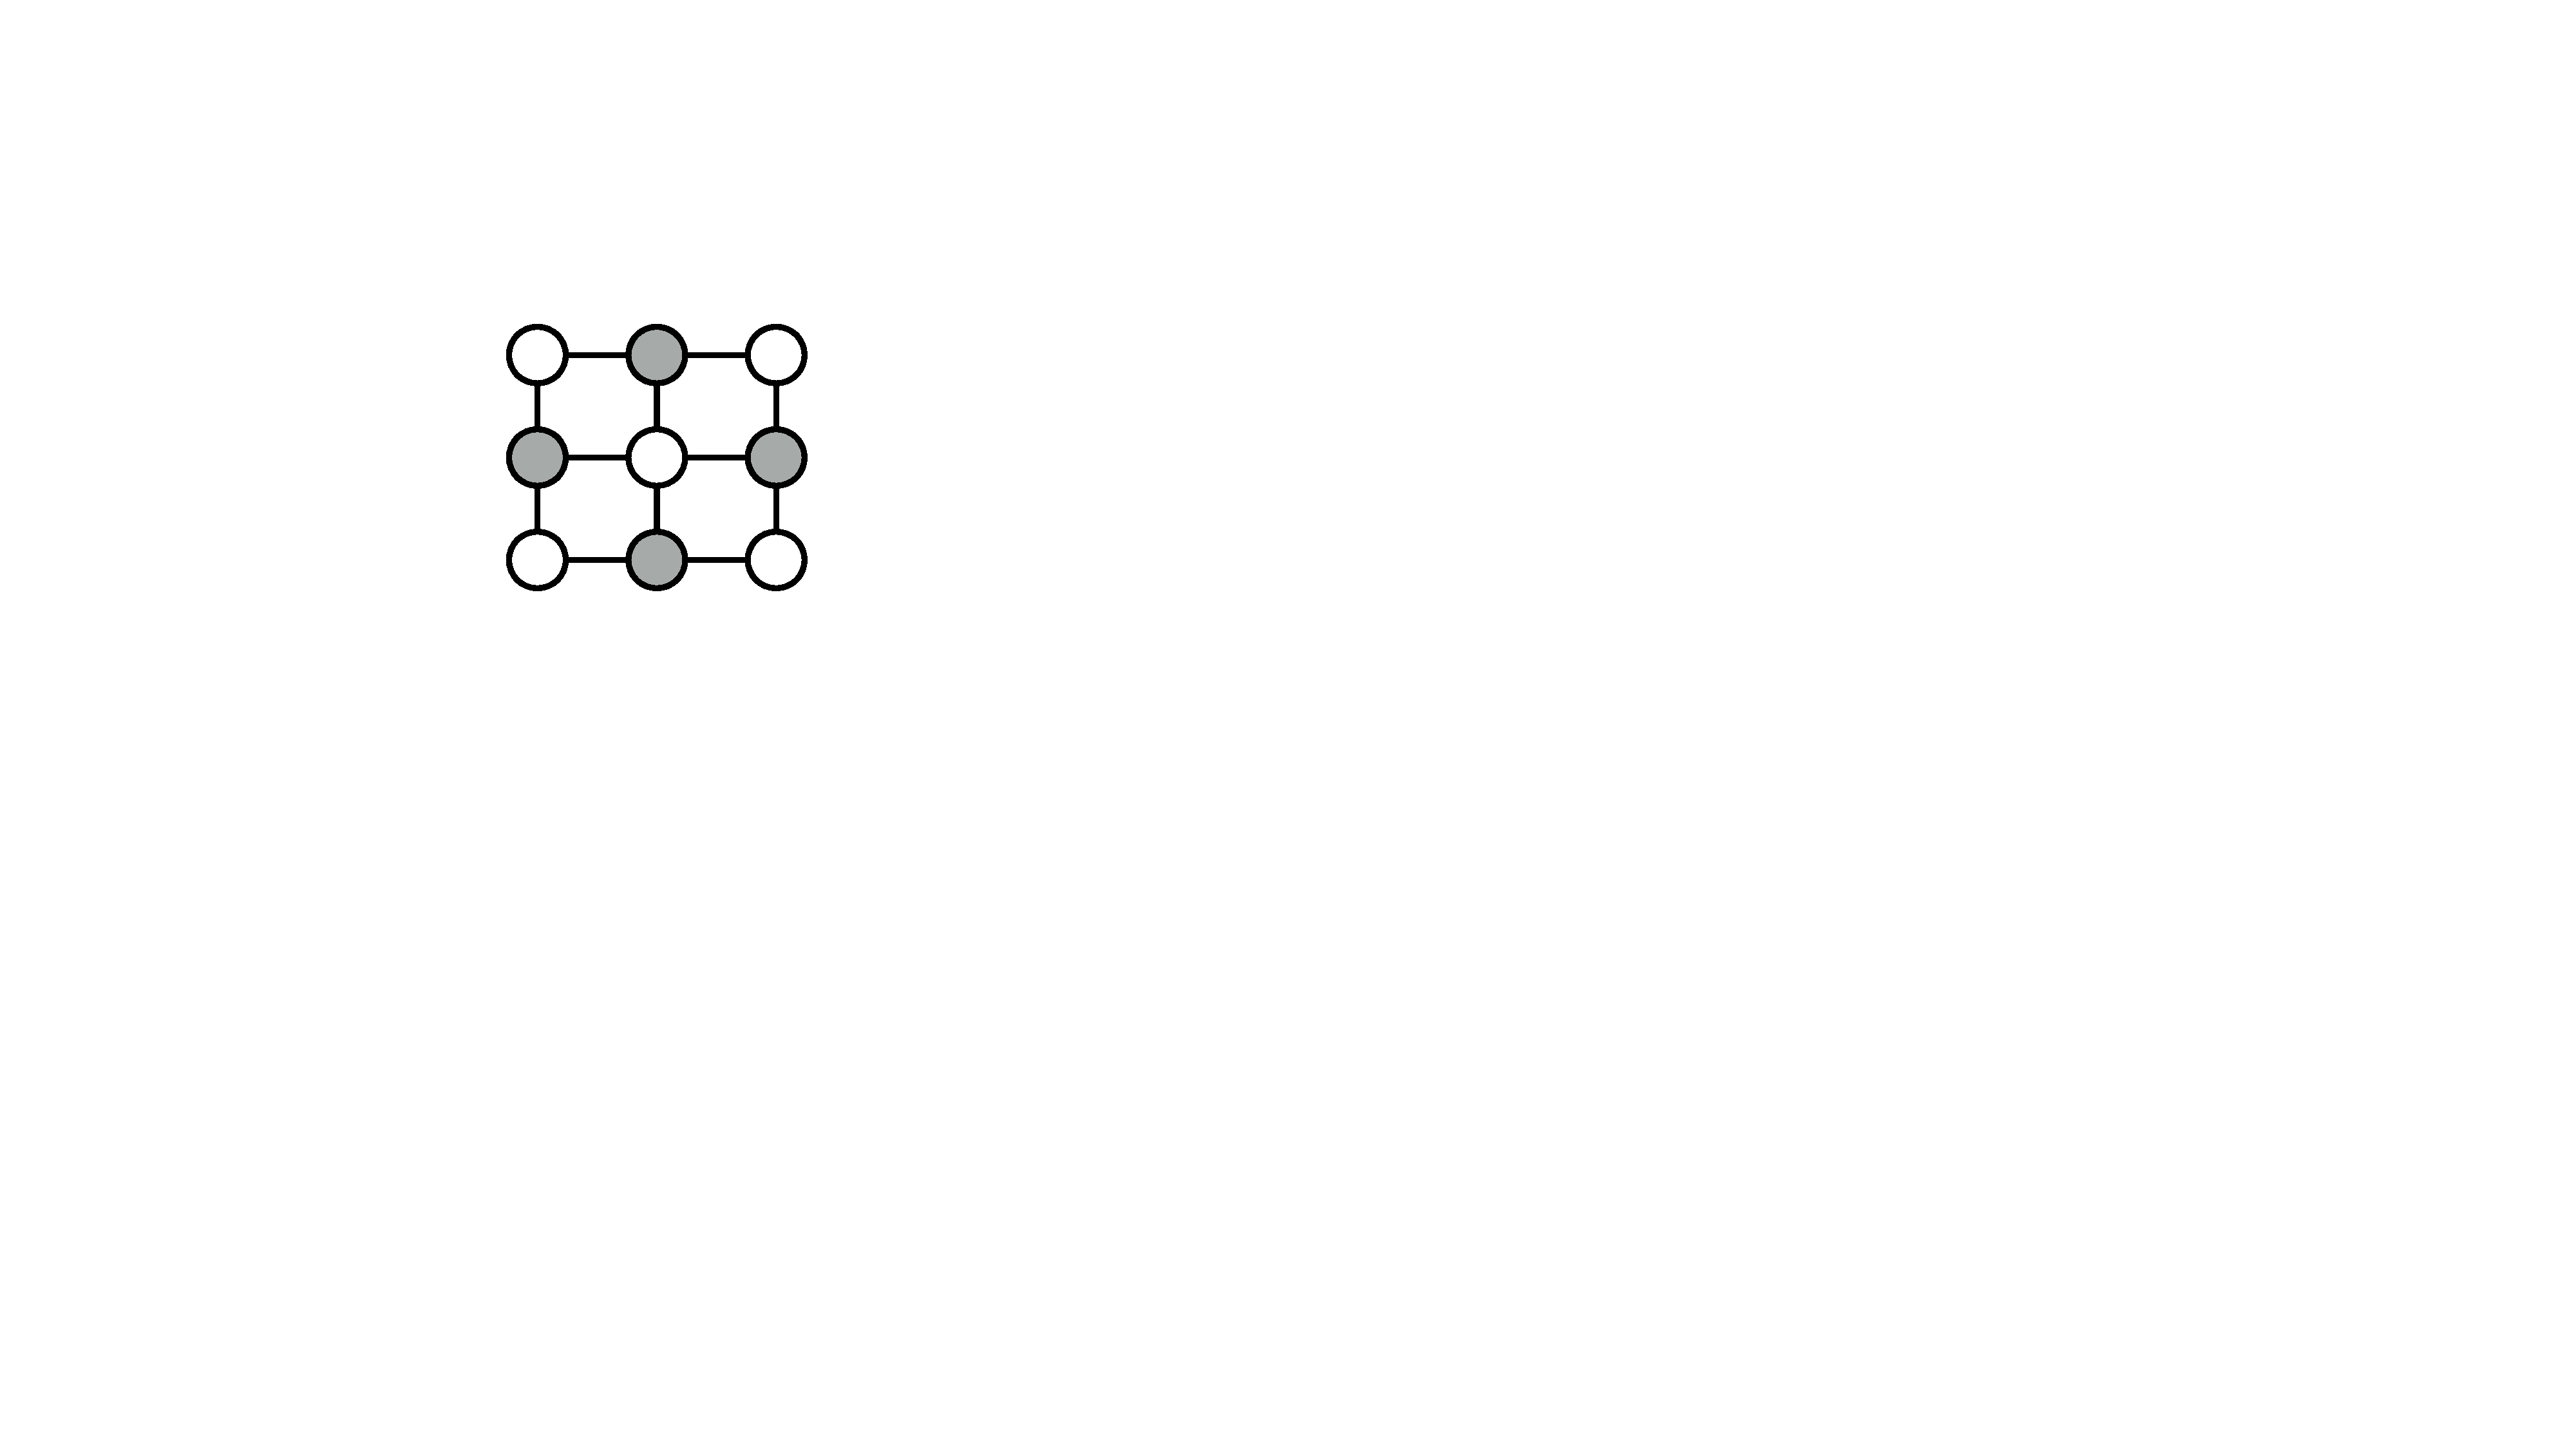
\includegraphics[height=0.2\paperheight]{ch-hvm/fig/markov-blanket-ising.pdf}
  \caption[Markov blanket of a random variable in an Ising model]{
  \textbf{The Markov blanket of a node in an Ising model consists of the node's nearest neighbors (nodes in the Markov blanket of the central node are shaded).} Conditioning on the Markov blanket of a node in a graphical model renders it conditionally independent of the rest of the variables. This enables building efficient variational approximations.}
  \label{fig:markov-blanket-ising}
\end{figure}

For studying a model $p(\mbx, \mbz)$, the variational family defined by an \gls{hvm} is defined as
\begin{equation}
  q_\hvm(\mbz; \mbtheta) = \int q(\mbnu; \mbtheta) \prod_i q(\mbz_i \mid \mbnu_i) d\mbnu \, ,
  \label{eq:hvm}
\end{equation}
where $q_\mf(\mbz \mid \mbnu) = \prod_i q(\mbz_i \mid \mbnu_i)$ is the mean field `variational likelihood' with parameters $\mbnu$, and $q(\mbnu; \mbtheta)$ is the variational prior with parameters $\mbtheta$. \Cref{fig:graphical-model} shows the graphical model for \glspl{hvm} as compared to the mean field family graphical model.

To use an \gls{hvm} in \gls{vi}, the variational lower bound must be optimized. But the variational lower bound in \Cref{eq:llbo} requires calculating the entropy of the variational distribution, and such integration in high dimensions can be intractable. As detailed in \citet{ranganath2018black}, the entropy can be lower-bounded by introducing an auxiliary `variational posterior' distribution $r(\mbnu \mid \mbz; \mbphi)$ with parameters $\mbphi$. This leads to the hierarchical evidence lower bound,
\begin{equation}
  \widetilde{{\cL}}(\mbtheta, \mbphi) = \E_{q(\mbz, \mbnu; \mbtheta)}[ \log p(\mbx, \mbz) + \log r(\mbnu \mid \mbz; \mbphi) - \log q(\mbz \mid \mbnu) - \log q(\mbnu; \mbtheta)]\, ,
  \label{eq:hier-elbo}
\end{equation}
and a stochastic optimization algorithm for this objective is developed in \citep{ranganath2018black}. \gls{vi} with an \gls{hvm} requires specifying the variational prior $q(\mbnu; \mbtheta)$ and the variational posterior ${r(\mbnu \mid \mbz; \mbphi)}$, then optimizing the hierarchical \gls{elbo} in \Cref{eq:hier-elbo}.

\paragraph{Specifying an \gls{hvm} with Normalizing Flows.} We study several choices of variational prior and recursive variational posterior. One choice of variational prior $q(\mbnu; \mbtheta)$ is an inverse autoregressive flow~\citep{kingma2016improved}. If the variational posterior $r(\mbnu \mid \mbz; \mbphi)$ is chosen to be a masked autoregressive flow~\citep{papamakarios2017masked}, the analytical forms of these flows are equivalent. These choices lead to a complexity of $\cO(L)$ for sampling latent variables in a system of size $L$. (This is because the noise used to sample from the variational prior can be drawn in parallel.) \glspl{hvm} should therefore be faster than \gls{van} approximations in large systems: the autoregressive requirement in \glspl{van} leads to a complexity of $\cO(L^2)$. A research question is whether the advantage in speed of \glspl{hvm} leads to a drop in accuracy that is too large to answer a statistical physics question.
% !TEX root = ../../main.tex
\begin{figure*}[t]
  \centering
  % adjust margin to center captions
  \captionsetup[subfigure]{margin={0cm,0cm},oneside}
  \hspace*{\fill}%
  \begin{subfigure}[c]{0.5\linewidth}
    \centering
    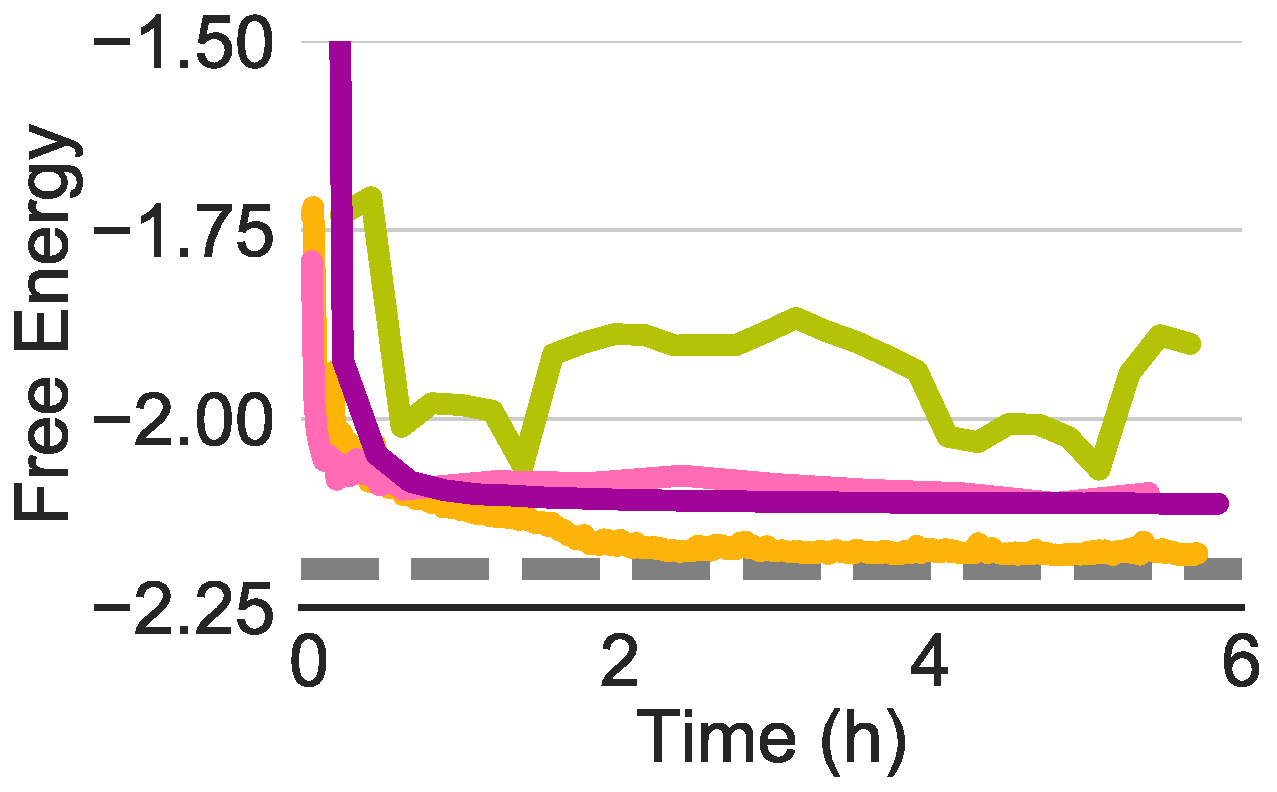
\includegraphics[width=\textwidth]{ch-hvm/fig/ising-large.pdf}
    % \caption{$\beta=0.4$}%
  \end{subfigure}
  % \hfill\hspace{\mywidth}%
  \begin{subfigure}[c]{0.3\linewidth}
    \centering
    % \raisebox{12mm}{
      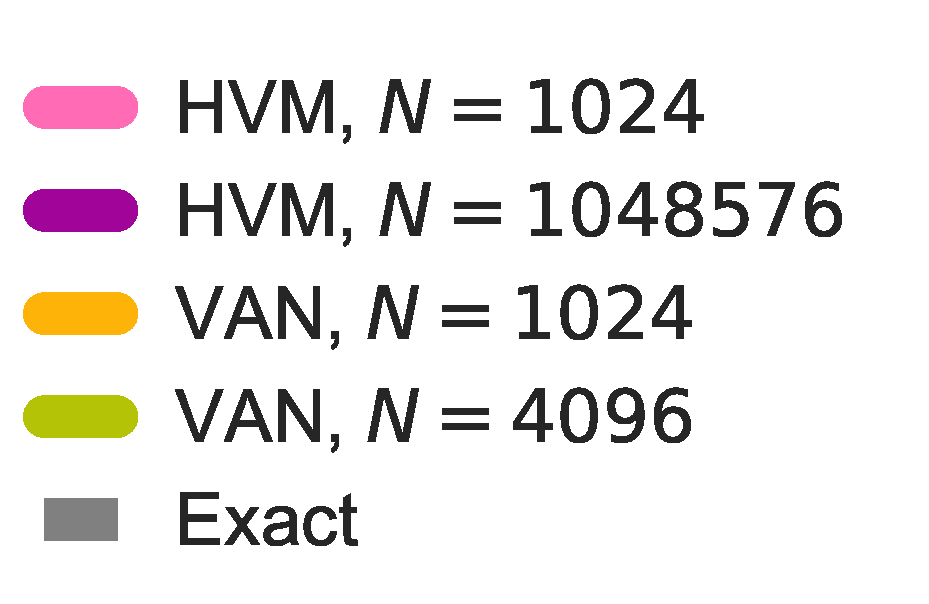
\includegraphics[width=\textwidth]{ch-hvm/fig/legend-ising}
    % }
  \end{subfigure}
  \hspace*{\fill}%
  % \vspace{-0.5cm}
  \caption[\textsc{hvm}s applied to the Ising model]{\textbf{\Acrfullpl{hvm} scale to statistical physics models with millions of random variables, with over 100x parameter savings.} The free energy is reported (the variational lower bound yields an upper bound on the free energy). The \gls{hvm} variational approximations use $5400$ parameters, while the \gls{van} method uses over $700$k.}
  \label{fig:hvm-ising}
\end{figure*}

\paragraph{Scalable \glspl{hvm} using Ising Model Structure.} Although \glspl{hvm} with autoregressive flows scale linearly, such variational approximations do not leverage the structure about the statistical physics under study. For example, it is difficult to index random variables so that nearest neighbors are grouped together when fed to an autoregressive model. However, consider the Markov blanket of a random variable in the Ising model---it contains all the information needed to render a variable conditionally independent of the rest of the model. The Markov blanket of a node in an Ising model consists of a node's nearest neighbors and is shown in \Cref{fig:markov-blanket-ising}. This means that an autoregressive model is overparameterized. For example, the last variable to be fed to the model depends on all the previous in an autoregressive model, whereas an efficient model might only consider nodes in a Markov blanket. A convenient way to build this structure into an \gls{hvm} would ensure efficient use of information from nearest neighbors in the Ising model. One way to formalize this problem structure is with convolutional neural networks~\citep{lecun2015deep}. We parameterize the variational prior and recursive posterior with \gls{realnvp} transformations using a convolutional neural network architecture \citep{dinh2017density}. Specifically, we parameterize the convolutional kernels to mimic the Markov blanket shown in \Cref{fig:markov-blanket-ising}: for every node, only its nearest neighbors are conditioned on.